\documentclass[]{article}
\usepackage{lmodern}
\usepackage{amssymb,amsmath}
\usepackage{ifxetex,ifluatex}
\usepackage{fixltx2e} % provides \textsubscript
\ifnum 0\ifxetex 1\fi\ifluatex 1\fi=0 % if pdftex
  \usepackage[T1]{fontenc}
  \usepackage[utf8]{inputenc}
\else % if luatex or xelatex
  \ifxetex
    \usepackage{mathspec}
  \else
    \usepackage{fontspec}
  \fi
  \defaultfontfeatures{Ligatures=TeX,Scale=MatchLowercase}
\fi
% use upquote if available, for straight quotes in verbatim environments
\IfFileExists{upquote.sty}{\usepackage{upquote}}{}
% use microtype if available
\IfFileExists{microtype.sty}{%
\usepackage{microtype}
\UseMicrotypeSet[protrusion]{basicmath} % disable protrusion for tt fonts
}{}
\usepackage[margin=2.54cm]{geometry}
\usepackage{hyperref}
\hypersetup{unicode=true,
            pdftitle={17: Crafting Reports},
            pdfauthor={Environmental Data Analytics \textbar{} Kateri Salk},
            pdfborder={0 0 0},
            breaklinks=true}
\urlstyle{same}  % don't use monospace font for urls
\usepackage{color}
\usepackage{fancyvrb}
\newcommand{\VerbBar}{|}
\newcommand{\VERB}{\Verb[commandchars=\\\{\}]}
\DefineVerbatimEnvironment{Highlighting}{Verbatim}{commandchars=\\\{\}}
% Add ',fontsize=\small' for more characters per line
\usepackage{framed}
\definecolor{shadecolor}{RGB}{248,248,248}
\newenvironment{Shaded}{\begin{snugshade}}{\end{snugshade}}
\newcommand{\KeywordTok}[1]{\textcolor[rgb]{0.13,0.29,0.53}{\textbf{#1}}}
\newcommand{\DataTypeTok}[1]{\textcolor[rgb]{0.13,0.29,0.53}{#1}}
\newcommand{\DecValTok}[1]{\textcolor[rgb]{0.00,0.00,0.81}{#1}}
\newcommand{\BaseNTok}[1]{\textcolor[rgb]{0.00,0.00,0.81}{#1}}
\newcommand{\FloatTok}[1]{\textcolor[rgb]{0.00,0.00,0.81}{#1}}
\newcommand{\ConstantTok}[1]{\textcolor[rgb]{0.00,0.00,0.00}{#1}}
\newcommand{\CharTok}[1]{\textcolor[rgb]{0.31,0.60,0.02}{#1}}
\newcommand{\SpecialCharTok}[1]{\textcolor[rgb]{0.00,0.00,0.00}{#1}}
\newcommand{\StringTok}[1]{\textcolor[rgb]{0.31,0.60,0.02}{#1}}
\newcommand{\VerbatimStringTok}[1]{\textcolor[rgb]{0.31,0.60,0.02}{#1}}
\newcommand{\SpecialStringTok}[1]{\textcolor[rgb]{0.31,0.60,0.02}{#1}}
\newcommand{\ImportTok}[1]{#1}
\newcommand{\CommentTok}[1]{\textcolor[rgb]{0.56,0.35,0.01}{\textit{#1}}}
\newcommand{\DocumentationTok}[1]{\textcolor[rgb]{0.56,0.35,0.01}{\textbf{\textit{#1}}}}
\newcommand{\AnnotationTok}[1]{\textcolor[rgb]{0.56,0.35,0.01}{\textbf{\textit{#1}}}}
\newcommand{\CommentVarTok}[1]{\textcolor[rgb]{0.56,0.35,0.01}{\textbf{\textit{#1}}}}
\newcommand{\OtherTok}[1]{\textcolor[rgb]{0.56,0.35,0.01}{#1}}
\newcommand{\FunctionTok}[1]{\textcolor[rgb]{0.00,0.00,0.00}{#1}}
\newcommand{\VariableTok}[1]{\textcolor[rgb]{0.00,0.00,0.00}{#1}}
\newcommand{\ControlFlowTok}[1]{\textcolor[rgb]{0.13,0.29,0.53}{\textbf{#1}}}
\newcommand{\OperatorTok}[1]{\textcolor[rgb]{0.81,0.36,0.00}{\textbf{#1}}}
\newcommand{\BuiltInTok}[1]{#1}
\newcommand{\ExtensionTok}[1]{#1}
\newcommand{\PreprocessorTok}[1]{\textcolor[rgb]{0.56,0.35,0.01}{\textit{#1}}}
\newcommand{\AttributeTok}[1]{\textcolor[rgb]{0.77,0.63,0.00}{#1}}
\newcommand{\RegionMarkerTok}[1]{#1}
\newcommand{\InformationTok}[1]{\textcolor[rgb]{0.56,0.35,0.01}{\textbf{\textit{#1}}}}
\newcommand{\WarningTok}[1]{\textcolor[rgb]{0.56,0.35,0.01}{\textbf{\textit{#1}}}}
\newcommand{\AlertTok}[1]{\textcolor[rgb]{0.94,0.16,0.16}{#1}}
\newcommand{\ErrorTok}[1]{\textcolor[rgb]{0.64,0.00,0.00}{\textbf{#1}}}
\newcommand{\NormalTok}[1]{#1}
\usepackage{longtable,booktabs}
\usepackage{graphicx,grffile}
\makeatletter
\def\maxwidth{\ifdim\Gin@nat@width>\linewidth\linewidth\else\Gin@nat@width\fi}
\def\maxheight{\ifdim\Gin@nat@height>\textheight\textheight\else\Gin@nat@height\fi}
\makeatother
% Scale images if necessary, so that they will not overflow the page
% margins by default, and it is still possible to overwrite the defaults
% using explicit options in \includegraphics[width, height, ...]{}
\setkeys{Gin}{width=\maxwidth,height=\maxheight,keepaspectratio}
\IfFileExists{parskip.sty}{%
\usepackage{parskip}
}{% else
\setlength{\parindent}{0pt}
\setlength{\parskip}{6pt plus 2pt minus 1pt}
}
\setlength{\emergencystretch}{3em}  % prevent overfull lines
\providecommand{\tightlist}{%
  \setlength{\itemsep}{0pt}\setlength{\parskip}{0pt}}
\setcounter{secnumdepth}{0}
% Redefines (sub)paragraphs to behave more like sections
\ifx\paragraph\undefined\else
\let\oldparagraph\paragraph
\renewcommand{\paragraph}[1]{\oldparagraph{#1}\mbox{}}
\fi
\ifx\subparagraph\undefined\else
\let\oldsubparagraph\subparagraph
\renewcommand{\subparagraph}[1]{\oldsubparagraph{#1}\mbox{}}
\fi

%%% Use protect on footnotes to avoid problems with footnotes in titles
\let\rmarkdownfootnote\footnote%
\def\footnote{\protect\rmarkdownfootnote}

%%% Change title format to be more compact
\usepackage{titling}

% Create subtitle command for use in maketitle
\newcommand{\subtitle}[1]{
  \posttitle{
    \begin{center}\large#1\end{center}
    }
}

\setlength{\droptitle}{-2em}

  \title{17: Crafting Reports}
    \pretitle{\vspace{\droptitle}\centering\huge}
  \posttitle{\par}
    \author{Environmental Data Analytics \textbar{} Kateri Salk}
    \preauthor{\centering\large\emph}
  \postauthor{\par}
      \predate{\centering\large\emph}
  \postdate{\par}
    \date{Spring 2019}


\begin{document}
\maketitle

\subsection{LESSON OBJECTIVES}\label{lesson-objectives}

\begin{enumerate}
\def\labelenumi{\arabic{enumi}.}
\tightlist
\item
  Describe the purpose of using R Markdown as a communication and
  workflow tool
\item
  Incorporate Markdown syntax into documents
\item
  Communicate the process and findings of an analysis session in the
  style of a report
\end{enumerate}

\subsection{BASIC R MARKDOWN DOCUMENT
STRUCTURE}\label{basic-r-markdown-document-structure}

\begin{enumerate}
\def\labelenumi{\arabic{enumi}.}
\tightlist
\item
  \textbf{YAML Header} surrounded by --- on top and bottom

  \begin{itemize}
  \tightlist
  \item
    YAML templates include options for html, pdf, word, markdown, and
    interactive
  \item
    More information on formatting the YAML header can be found in the
    cheat sheet
  \end{itemize}
\item
  \textbf{R Code Chunks} surrounded by
  ``\texttt{on\ top\ and\ bottom\ +\ Create\ using}Cmd/Ctrl\texttt{+}Alt\texttt{+}I`

  \begin{itemize}
  \tightlist
  \item
    Can be named \{r name\} to facilitate navigation and autoreferencing
  \item
    Chunk options allow for flexibility when the code runs and when the
    document is knitted
  \end{itemize}
\item
  \textbf{Text} with formatting options for readability in knitted
  document
\end{enumerate}

A handy cheat sheet for R markdown can be found
\href{https://www.rstudio.com/wp-content/uploads/2015/03/rmarkdown-reference.pdf}{here}.
Another one can be found
\href{https://www.rstudio.com/wp-content/uploads/2015/02/rmarkdown-cheatsheet.pdf}{here}.

\subsection{WHY R MARKDOWN?}\label{why-r-markdown}

 need to add space after, additional return between paragraph

\begin{itemize}
\tightlist
\item
  Code, output, text, and notes in one document
\item
  Knit to useful formats
\item
  Legible code \_ output
\item
  Git friendly - version control!
\item
  Reproducible
\item
  Updating capacilities
\item
  Focus on output and conclusions, not code (flexible formating)
\end{itemize}

\subsection{TEXT EDITING CHALLENGE}\label{text-editing-challenge}

Create a table below that details the example datasets we have been
using in class. The first column should contain the name of the dataset
and the second column should include some relevant information about the
dataset. the dashes difine the width of the table

\begin{longtable}[]{@{}ll@{}}
\toprule
Dataset & Information\tabularnewline
\midrule
\endhead
item & info\tabularnewline
\bottomrule
\end{longtable}

\subsection{R CHUNK EDITING CHALLENGE}\label{r-chunk-editing-challenge}

\subsubsection{Installing packages}\label{installing-packages}

Create an R chunk below that installs the package \texttt{knitr}.
Instead of commenting out the code, customize the chunk options such
that the code is not evaluated (i.e., not run).

\begin{Shaded}
\begin{Highlighting}[]
\KeywordTok{install.packages}\NormalTok{(}\StringTok{"knitr"}\NormalTok{)}
\end{Highlighting}
\end{Shaded}

\subsubsection{Setup}\label{setup}

Create an R chunk below called ``setup'' that checks your working
directory, loads the packages \texttt{tidyverse} and \texttt{knitr}, and
sets a ggplot theme.

\begin{Shaded}
\begin{Highlighting}[]
\KeywordTok{getwd}\NormalTok{()}
\end{Highlighting}
\end{Shaded}

\begin{verbatim}
## [1] "/Users/Sylvia/Downloads/ENV872/ENV872"
\end{verbatim}

\begin{Shaded}
\begin{Highlighting}[]
\KeywordTok{library}\NormalTok{(tidyverse)}
\end{Highlighting}
\end{Shaded}

\begin{verbatim}
## -- Attaching packages ---------------------------------------------------------------------- tidyverse 1.2.1 --
\end{verbatim}

\begin{verbatim}
## v ggplot2 3.1.0       v purrr   0.2.5  
## v tibble  2.0.1       v dplyr   0.8.0.1
## v tidyr   0.8.2       v stringr 1.3.1  
## v readr   1.3.1       v forcats 0.3.0
\end{verbatim}

\begin{verbatim}
## -- Conflicts ------------------------------------------------------------------------- tidyverse_conflicts() --
## x dplyr::filter() masks stats::filter()
## x dplyr::lag()    masks stats::lag()
\end{verbatim}

\begin{Shaded}
\begin{Highlighting}[]
\KeywordTok{library}\NormalTok{(knitr)}
\NormalTok{mytheme <-}\StringTok{ }\KeywordTok{theme_bw}\NormalTok{(}\DataTypeTok{base_size =} \DecValTok{14}\NormalTok{) }\OperatorTok{+}
\StringTok{  }\KeywordTok{theme}\NormalTok{(}\DataTypeTok{axis.text =} \KeywordTok{element_text}\NormalTok{(}\DataTypeTok{color =} \StringTok{"black"}\NormalTok{), }
        \DataTypeTok{legend.position =} \StringTok{"bottom"}\NormalTok{,}
        \DataTypeTok{panel.grid.major =} \KeywordTok{element_line}\NormalTok{(}\DataTypeTok{size =} \FloatTok{0.5}\NormalTok{, }\DataTypeTok{linetype =} \StringTok{'solid'}\NormalTok{), }
        \DataTypeTok{panel.grid.minor =} \KeywordTok{element_line}\NormalTok{(}\DataTypeTok{size =} \FloatTok{0.25}\NormalTok{, }\DataTypeTok{linetype =} \StringTok{'dashed'}\NormalTok{),}
        \DataTypeTok{title =} \KeywordTok{element_text}\NormalTok{(}\DataTypeTok{face =} \StringTok{"bold"}\NormalTok{))}
\KeywordTok{theme_set}\NormalTok{(mytheme)}
\end{Highlighting}
\end{Shaded}

Load the NTL-LTER\_Lake\_Nutrients\_Raw dataset, display the head of the
dataset, and set the date column to a date format.

Customize the chunk options such that the code is run but is not
displayed in the final document.

\begin{verbatim}
##   lakeid  lakename year4 daynum sampledate depth_id depth tn_ug tp_ug nh34
## 1      L Paul Lake  1991    140    5/20/91        1  0.00   538    25   NA
## 2      L Paul Lake  1991    140    5/20/91        2  0.85   285    14   NA
## 3      L Paul Lake  1991    140    5/20/91        3  1.75   399    14   NA
## 4      L Paul Lake  1991    140    5/20/91        4  3.00   453    14   NA
## 5      L Paul Lake  1991    140    5/20/91        5  4.00   363    13   NA
## 6      L Paul Lake  1991    140    5/20/91        6  6.00   583    37   NA
##   no23 po4 comments
## 1   NA  NA         
## 2   NA  NA         
## 3   NA  NA         
## 4   NA  NA         
## 5   NA  NA         
## 6   NA  NA
\end{verbatim}

\subsubsection{Data Exploration, Wrangling, and
Visualization}\label{data-exploration-wrangling-and-visualization}

Create an R chunk below to create a processed dataset do the following
operations:

\begin{itemize}
\tightlist
\item
  Include all columns except lakeid, depth\_id, and comments
\item
  Include only surface samples (depth = 0 m)
\end{itemize}

Create a second R chunk to create a summary dataset with the mean,
minimum, maximum, and standard deviation of total nitrogen
concentrations for each lake. Create a second summary dataset that is
identical except that it evaluates total phosphorus. Customize the chunk
options such that the code is run but not displayed in the final
document.

Create a third R chunk that uses the function \texttt{kable} in the
knitr package to display two tables: one for the summary dataframe for
total N and one for the summary dataframe of total P. Use the
\texttt{caption\ =\ "\ "} code within that function to title your
tables. Customize the chunk options such that the final table is
displayed but not the code used to generate the table.

\begin{longtable}[]{@{}lrrrr@{}}
\caption{Total N summary}\tabularnewline
\toprule
lakename & meanTN & minTN & maxTN & sdTN\tabularnewline
\midrule
\endfirsthead
\toprule
lakename & meanTN & minTN & maxTN & sdTN\tabularnewline
\midrule
\endhead
Central Long Lake & 690.0469 & 343.020 & 953.063 &
209.09341\tabularnewline
Crampton Lake & 362.6813 & 353.380 & 376.304 & 12.05748\tabularnewline
East Long Lake & 810.7834 & 380.620 & 2608.956 &
335.41457\tabularnewline
Hummingbird Lake & 1036.6695 & 779.053 & 1221.960 &
204.36889\tabularnewline
Paul Lake & 368.7564 & 45.670 & 628.625 & 106.34741\tabularnewline
Peter Lake & 561.8752 & 219.720 & 2048.151 & 305.64909\tabularnewline
Tuesday Lake & 423.5605 & 237.363 & 554.418 & 78.84522\tabularnewline
West Long Lake & 762.6017 & 303.170 & 2870.302 &
402.95992\tabularnewline
\bottomrule
\end{longtable}

\begin{longtable}[]{@{}lrrrr@{}}
\caption{Total P summary}\tabularnewline
\toprule
lakename & meanTP & minTP & maxTP & sdTP\tabularnewline
\midrule
\endfirsthead
\toprule
lakename & meanTP & minTP & maxTP & sdTP\tabularnewline
\midrule
\endhead
Central Long Lake & 21.70981 & 8.190 & 37.270 & 7.076388\tabularnewline
Crampton Lake & 11.16033 & 5.803 & 15.555 & 4.946759\tabularnewline
East Long Lake & 29.28984 & 8.000 & 101.050 & 17.375710\tabularnewline
Hummingbird Lake & 36.21925 & 32.765 & 42.119 & 4.146717\tabularnewline
Paul Lake & 10.45606 & 1.222 & 36.070 & 4.805142\tabularnewline
Peter Lake & 18.39153 & 0.000 & 64.383 & 10.976205\tabularnewline
Tuesday Lake & 11.71853 & 6.325 & 18.663 & 3.044289\tabularnewline
West Long Lake & 19.82981 & 2.690 & 63.243 & 10.541276\tabularnewline
\bottomrule
\end{longtable}

Create a fourth and fifth R chunk that generates two plots (one in each
chunk): one for total N over time with different colors for each lake,
and one with the same setup but for total P. Decide which geom option
will be appropriate for your purpose, and select a color palette that is
visually pleasing and accessible. Customize the chunk options such that
the final figures are displayed but not the code used to generate the
figures. In addition, customize the chunk options such that the figures
are aligned on the left side of the page. Lastly, add a fig.cap chunk
option to add a caption (title) to your plot that will display
underneath the figure.

\begin{verbatim}
## `geom_smooth()` using method = 'loess' and formula 'y ~ x'
\end{verbatim}

\begin{verbatim}
## Warning: Removed 139 rows containing non-finite values (stat_smooth).
\end{verbatim}

\begin{verbatim}
## Warning in simpleLoess(y, x, w, span, degree = degree, parametric =
## parametric, : span too small. fewer data values than degrees of freedom.
\end{verbatim}

\begin{verbatim}
## Warning in simpleLoess(y, x, w, span, degree = degree, parametric =
## parametric, : pseudoinverse used at 10753
\end{verbatim}

\begin{verbatim}
## Warning in simpleLoess(y, x, w, span, degree = degree, parametric =
## parametric, : neighborhood radius 34.35
\end{verbatim}

\begin{verbatim}
## Warning in simpleLoess(y, x, w, span, degree = degree, parametric =
## parametric, : reciprocal condition number 0
\end{verbatim}

\begin{verbatim}
## Warning in simpleLoess(y, x, w, span, degree = degree, parametric =
## parametric, : There are other near singularities as well. 1321.3
\end{verbatim}

\begin{verbatim}
## Warning in predLoess(object$y, object$x, newx = if
## (is.null(newdata)) object$x else if (is.data.frame(newdata))
## as.matrix(model.frame(delete.response(terms(object)), : span too small.
## fewer data values than degrees of freedom.
\end{verbatim}

\begin{verbatim}
## Warning in predLoess(object$y, object$x, newx = if
## (is.null(newdata)) object$x else if (is.data.frame(newdata))
## as.matrix(model.frame(delete.response(terms(object)), : pseudoinverse used
## at 10753
\end{verbatim}

\begin{verbatim}
## Warning in predLoess(object$y, object$x, newx = if
## (is.null(newdata)) object$x else if (is.data.frame(newdata))
## as.matrix(model.frame(delete.response(terms(object)), : neighborhood radius
## 34.35
\end{verbatim}

\begin{verbatim}
## Warning in predLoess(object$y, object$x, newx = if
## (is.null(newdata)) object$x else if (is.data.frame(newdata))
## as.matrix(model.frame(delete.response(terms(object)), : reciprocal
## condition number 0
\end{verbatim}

\begin{verbatim}
## Warning in predLoess(object$y, object$x, newx = if
## (is.null(newdata)) object$x else if (is.data.frame(newdata))
## as.matrix(model.frame(delete.response(terms(object)), : There are other
## near singularities as well. 1321.3
\end{verbatim}

\begin{verbatim}
## Warning in simpleLoess(y, x, w, span, degree = degree, parametric =
## parametric, : span too small. fewer data values than degrees of freedom.
\end{verbatim}

\begin{verbatim}
## Warning in simpleLoess(y, x, w, span, degree = degree, parametric =
## parametric, : pseudoinverse used at 10736
\end{verbatim}

\begin{verbatim}
## Warning in simpleLoess(y, x, w, span, degree = degree, parametric =
## parametric, : neighborhood radius 56.42
\end{verbatim}

\begin{verbatim}
## Warning in simpleLoess(y, x, w, span, degree = degree, parametric =
## parametric, : reciprocal condition number 0
\end{verbatim}

\begin{verbatim}
## Warning in simpleLoess(y, x, w, span, degree = degree, parametric =
## parametric, : There are other near singularities as well. 3183.2
\end{verbatim}

\begin{verbatim}
## Warning in predLoess(object$y, object$x, newx = if
## (is.null(newdata)) object$x else if (is.data.frame(newdata))
## as.matrix(model.frame(delete.response(terms(object)), : span too small.
## fewer data values than degrees of freedom.
\end{verbatim}

\begin{verbatim}
## Warning in predLoess(object$y, object$x, newx = if
## (is.null(newdata)) object$x else if (is.data.frame(newdata))
## as.matrix(model.frame(delete.response(terms(object)), : pseudoinverse used
## at 10736
\end{verbatim}

\begin{verbatim}
## Warning in predLoess(object$y, object$x, newx = if
## (is.null(newdata)) object$x else if (is.data.frame(newdata))
## as.matrix(model.frame(delete.response(terms(object)), : neighborhood radius
## 56.42
\end{verbatim}

\begin{verbatim}
## Warning in predLoess(object$y, object$x, newx = if
## (is.null(newdata)) object$x else if (is.data.frame(newdata))
## as.matrix(model.frame(delete.response(terms(object)), : reciprocal
## condition number 0
\end{verbatim}

\begin{verbatim}
## Warning in predLoess(object$y, object$x, newx = if
## (is.null(newdata)) object$x else if (is.data.frame(newdata))
## as.matrix(model.frame(delete.response(terms(object)), : There are other
## near singularities as well. 3183.2
\end{verbatim}

\begin{figure}

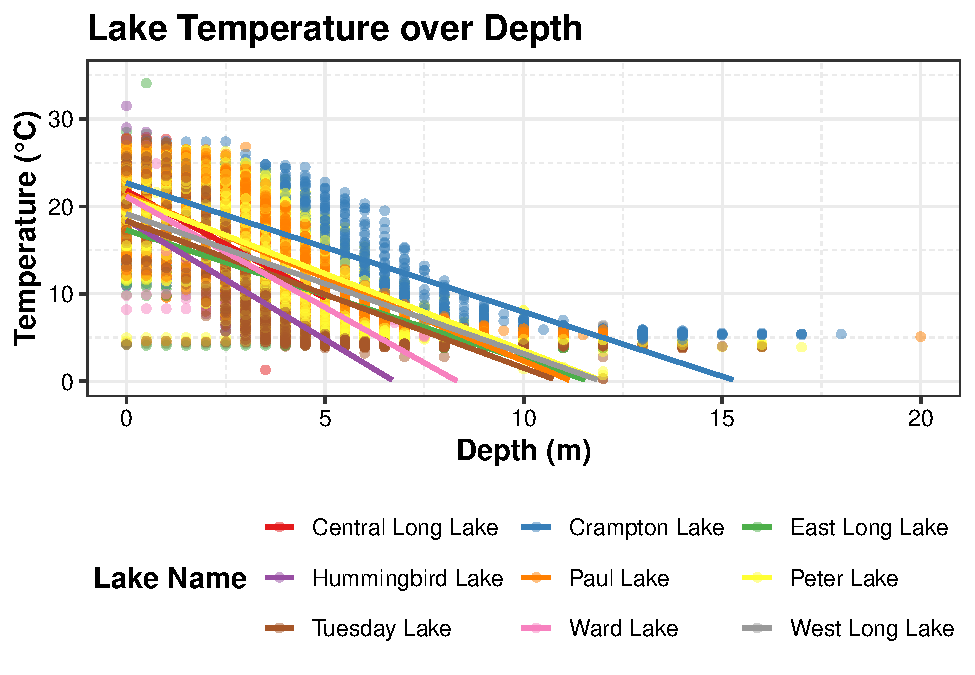
\includegraphics{17_CraftingReports_files/figure-latex/unnamed-chunk-6-1} \hfill{}

\caption{total N over time}\label{fig:unnamed-chunk-6}
\end{figure}

\begin{verbatim}
## `geom_smooth()` using method = 'loess' and formula 'y ~ x'
\end{verbatim}

\begin{verbatim}
## Warning: Removed 7 rows containing non-finite values (stat_smooth).
\end{verbatim}

\begin{verbatim}
## Warning in simpleLoess(y, x, w, span, degree = degree, parametric =
## parametric, : span too small. fewer data values than degrees of freedom.
\end{verbatim}

\begin{verbatim}
## Warning in simpleLoess(y, x, w, span, degree = degree, parametric =
## parametric, : pseudoinverse used at 10753
\end{verbatim}

\begin{verbatim}
## Warning in simpleLoess(y, x, w, span, degree = degree, parametric =
## parametric, : neighborhood radius 34.35
\end{verbatim}

\begin{verbatim}
## Warning in simpleLoess(y, x, w, span, degree = degree, parametric =
## parametric, : reciprocal condition number 0
\end{verbatim}

\begin{verbatim}
## Warning in simpleLoess(y, x, w, span, degree = degree, parametric =
## parametric, : There are other near singularities as well. 1321.3
\end{verbatim}

\begin{verbatim}
## Warning in predLoess(object$y, object$x, newx = if
## (is.null(newdata)) object$x else if (is.data.frame(newdata))
## as.matrix(model.frame(delete.response(terms(object)), : span too small.
## fewer data values than degrees of freedom.
\end{verbatim}

\begin{verbatim}
## Warning in predLoess(object$y, object$x, newx = if
## (is.null(newdata)) object$x else if (is.data.frame(newdata))
## as.matrix(model.frame(delete.response(terms(object)), : pseudoinverse used
## at 10753
\end{verbatim}

\begin{verbatim}
## Warning in predLoess(object$y, object$x, newx = if
## (is.null(newdata)) object$x else if (is.data.frame(newdata))
## as.matrix(model.frame(delete.response(terms(object)), : neighborhood radius
## 34.35
\end{verbatim}

\begin{verbatim}
## Warning in predLoess(object$y, object$x, newx = if
## (is.null(newdata)) object$x else if (is.data.frame(newdata))
## as.matrix(model.frame(delete.response(terms(object)), : reciprocal
## condition number 0
\end{verbatim}

\begin{verbatim}
## Warning in predLoess(object$y, object$x, newx = if
## (is.null(newdata)) object$x else if (is.data.frame(newdata))
## as.matrix(model.frame(delete.response(terms(object)), : There are other
## near singularities as well. 1321.3
\end{verbatim}

\begin{verbatim}
## Warning in simpleLoess(y, x, w, span, degree = degree, parametric =
## parametric, : span too small. fewer data values than degrees of freedom.
\end{verbatim}

\begin{verbatim}
## Warning in simpleLoess(y, x, w, span, degree = degree, parametric =
## parametric, : pseudoinverse used at 10736
\end{verbatim}

\begin{verbatim}
## Warning in simpleLoess(y, x, w, span, degree = degree, parametric =
## parametric, : neighborhood radius 56.42
\end{verbatim}

\begin{verbatim}
## Warning in simpleLoess(y, x, w, span, degree = degree, parametric =
## parametric, : reciprocal condition number 0
\end{verbatim}

\begin{verbatim}
## Warning in simpleLoess(y, x, w, span, degree = degree, parametric =
## parametric, : There are other near singularities as well. 3183.2
\end{verbatim}

\begin{verbatim}
## Warning in predLoess(object$y, object$x, newx = if
## (is.null(newdata)) object$x else if (is.data.frame(newdata))
## as.matrix(model.frame(delete.response(terms(object)), : span too small.
## fewer data values than degrees of freedom.
\end{verbatim}

\begin{verbatim}
## Warning in predLoess(object$y, object$x, newx = if
## (is.null(newdata)) object$x else if (is.data.frame(newdata))
## as.matrix(model.frame(delete.response(terms(object)), : pseudoinverse used
## at 10736
\end{verbatim}

\begin{verbatim}
## Warning in predLoess(object$y, object$x, newx = if
## (is.null(newdata)) object$x else if (is.data.frame(newdata))
## as.matrix(model.frame(delete.response(terms(object)), : neighborhood radius
## 56.42
\end{verbatim}

\begin{verbatim}
## Warning in predLoess(object$y, object$x, newx = if
## (is.null(newdata)) object$x else if (is.data.frame(newdata))
## as.matrix(model.frame(delete.response(terms(object)), : reciprocal
## condition number 0
\end{verbatim}

\begin{verbatim}
## Warning in predLoess(object$y, object$x, newx = if
## (is.null(newdata)) object$x else if (is.data.frame(newdata))
## as.matrix(model.frame(delete.response(terms(object)), : There are other
## near singularities as well. 3183.2
\end{verbatim}

\begin{figure}

\includegraphics{17_CraftingReports_files/figure-latex/unnamed-chunk-7-1} \hfill{}

\caption{total N over time}\label{fig:unnamed-chunk-7}
\end{figure}

\subsubsection{Other options}\label{other-options}

What are the chunk options that will suppress the display of errors,
warnings, and messages in the final document?

\begin{quote}
ANSWER:
\end{quote}

\subsubsection{Communicating results}\label{communicating-results}

Write a paragraph describing your findings from the R coding challenge
above. This should be geared toward an educated audience but one that is
not necessarily familiar with the dataset. Then insert a horizontal rule
below the paragraph. Below the horizontal rule, write another paragraph
describing the next steps you might take in analyzing this dataset. What
questions might you be able to answer, and what analyses would you
conduct to answer those questions?

\subsection{OTHER R MARKDOWN CUSTOMIZATION
OPTIONS}\label{other-r-markdown-customization-options}

We have covered the basics in class today, but R Markdown offers many
customization options. A word of caution: customizing templates will
often require more interaction with LaTeX and installations on your
computer, so be ready to troubleshoot issues.

Customization options for pdf output include:

\begin{itemize}
\tightlist
\item
  Table of contents
\item
  Number sections
\item
  Control default size of figures
\item
  Citations
\item
  Template (more info
  \href{http://jianghao.wang/post/2017-12-08-rmarkdown-templates/}{here})
\end{itemize}

pdf\_document:\\
toc: true\\
number\_sections: true\\
fig\_height: 3\\
fig\_width: 4\\
citation\_package: natbib\\
template:


\end{document}
